\chapter{Theorie}
\label{theory}

\section{CAP-Theorem}
\label{cap}

Um ein System zu entwerfen, das die Anforderungen erfüllt, ist es zunächst wichtig herauszufinden, welche Eigenschaften ein verteiltes System überhaupt theoretisch erfüllen kann. Dabei hilft das CAP-Theorem \cite{cap}. Es beweist, dass ein verteilter Speicher von den drei Eigenschaften 
\begin{itemize}
	\item \textbf{Konsistenz}: Wird von den Autoren als \textit{Linearizability} (auch \textit{Atomic Consistency}) definiert: Wenn ein Write abgeschlossen ist, müssen alle Reads, die danach beginnen, den Wert des Writes oder eines späteren Writes zurückgeben. Dies ist ein sehr starkes Konsistenzmodell.
	\item \textbf{Verfügbarkeit}: Das System ist zu jedem Zeitpunkt erreichbar und antwortet auf alle Anfragen an nicht abgestürzte Knoten.
	\item \textbf{Partitionstoleranz}: Das System funktioniert weiter falls das Netzwerk partitioniert wird, also ein Teil der Knoten von einem anderen Teil abgeschnitten ist.
\end{itemize}
 höchstens zwei gleichzeitig erfüllen kann. 

Konsistenz und Verfügbarkeit kann man als graduelle Eigenschaften ansehen. Im CAP-Theorem wird von einem sehr starken Konsistenzmodell ausgegangen, das sich je nach Anwendung auch lockern lässt. Ebenso kann man die Verfügbarkeit graduell anpassen. Es muss also abgewogen werden, welche dieser Eigenschaften für ein System wichtig sind und welche nicht. Deshalb kann es viele verschiedene System mit verschiedenen Eigenschaften für ganz unterschiedliche Einsatzgebiete geben. Partitionstoleranz ist in der Realtität wichtig, da man diese in typischen Einsatzorten wie Datenzentren nie ausschließen kann. Netzwerkpartitionierungen können z.B. durch Ausfälle von einzelnen Switches oder Routern hervorgerufen werden. 

Sehr viele verteilte Systeme sind auf hohe Verfügbarkeit optimiert, da sie z.B. ständig über das Internet erreichbar sein sollen. Darunter sind z.B. die meisten SQL- und NoSQL-Datenbanken und Key-Value-Stores wie DXRAM. SQL-Datenbanken wollen nach dem ACID-Prinzip möglich starke Konsistenz der Daten, weshalb sie meist die Partitionstoleranz aufgeben. NoSQL-Datenbanken lockern das Konsistenzmodell nach dem BASE-Prinzip und versuchen dadurch die Partitionstoleranz zu erreichen. Einige Systeme verwenden auch ein externes System um wichtige Daten, die auch bei einer Netzwerkpartitionierung noch konsistent vorhanden sein müssen, separat zu speichern. Dies ist ein Anwendungsgebiet für das System, das in dieser Arbeit entworfen werden soll.

Ein weiteres Beispiel für ein System, welches die Konsistenz zugunsten der Verfügbarkeit und der Partitionstoleranz abschwächt, ist das Domain Name System (DNS). Die DNS-Einträge werden auf den Nameservern für eine bestimmte Zeit zwischengespeichert, um Verfügbarkeit und Partitionstoleranz zu erreichen. Dadurch ist es jedoch möglich, dass diese Caches nicht aktuell und somit nicht konsistent zu ihren Ursprüngen sind.

Besonders wichtig für das System, das in dieser Arbeit entworfen werden soll, ist die Konsistenz. Alle Knoten im verteilten System sollten stets die gleiche Sicht auf den Status haben, sodass sie sich koordinieren und auf bestimmte Dinge einigen können. Dafür muss gerade die \textit{Atomic Consistency} erreicht werden, die auch im CAP-Theorem verwendet wird.

Um Konsistenz in einem verteilten System zu erreichen, muss das fundamentale Problem der Einigung auf einen Wert (oder einer Sequenz von Werten) gelöst werden. Wenn sich alle Knoten eines verteilten Systems auf den gleichen Wert geeinigt haben und dieser für alle sichtbar ist, dann ist das System für alle Knoten konsistent. Algorithmen, die dies ermöglichen, nennt man deshalb \textit{Einigungsalgorithmen}.

Da das Problem im Allgemeinen nicht trivial ist, sollen im Folgenden ein paar Algorithmen vorgestellt werden, die das Problem mit vereinfachten Modellen, die meist nicht den realen Bedingungen entsprechen, lösen.

\subsection{Flooding Consensus}

Der Flooding Consensus Algorithmus löst das Einigungsproblem in einem synchronen System und mit einem Fail-Stop-Modell, d.h. Server können abstürzen und senden dann keine Nachrichten mehr. Der Algorithmus läuft in \textit{n} Runden ab. Jeder Server hat zu Beginn einen Wert und speichert sich die gesamte Liste der empfangenen Werte. In jeder Runde flutet jeder Server das Netzwerk mit seinen bekannten Werten, d.h. er sendet seine Liste an alle teilnehmenden Server. Falls in einer Runde mindestens ein Server beim Senden oder vor dem Senden ausfällt, kann in dieser Runde keine Einigung erreicht werden, da es sein kann, dass die Server unterschiedliche Werte in ihren Listen haben. Um \textit{f} fehlerhafte Server zu kompensieren, werden also maximal \textit{f+1} Runden benötigt, bis die Server alle die gleichen Werte in ihren Listen haben. Dann können sie mit einer Funktion, die auf der Liste ausgeführt wird, den Entscheidungswert bestimmen. Dies könnte z.B. die Maximumsfunktion sein.
Um festzustellen, wann eine Runde vorbei ist, muss die maximale Nachrichtenlaufzeit und die maximale Bearbeitungszeit bekannt sein. Wenn dies bekannt ist, können die Server in jeder Runde diese Zeit abwarten und es ist sicher, dass ein Server, von dem in dieser Zeit keine Nachricht erhalten wurde, abgestürzt ist. Da man diese Zeit in der Praxis jedoch normalerweise nicht bestimmen kann, ist dieser Algorithmus meistens nicht für einen Einsatz geeignet.

\subsection{2-Phase-Commit}

Der 2-Phase-Commit-Algorithmus löst das Einigungsproblem in einem asynchronen System mit einer perfekten Ausfallerkennung. Hier geschieht die Einigung mithilfe eines Koordinators, der vorher mit einem externen Verfahren bestimmt werden muss, z.B. einem Leader-Election-Algorithmus. Da der Koordinator auch ausfallen kann und ein neuer Koordinator einen inkonsistenten Wert verbreiten könnte, kann dieser nicht einfach alle Werte einsammeln und entscheiden, sondern der Algorithmus muss in zwei Phasen durchgeführt werden:

\begin{itemize}
	\item \textbf{Phase 1}: Der Koordinator sendet eine \textit{propose}-Nachricht an alle Server mit seinem Wert, auf den sich geeinigt werden soll. Die Server akzeptieren den vorgeschlagenen Wert und merken sich diesen. Der Koordinator wartet auf Antworten von allen nicht ausgefallenen Servern (hier wird die Ausfallerkennung benötigt). Sobald er von allen Servern eine Antwort erhalten hat, ist es sicher, dass ein möglicher neuer Koordinator denselben Wert verbreiten wird, falls dieser Koordinator ausfällt. Die Aktivierung eines neuen Koordinators kann ebenfalls nur durch die perfekte Ausfallerkennung erreicht werden, sonst kann es sein, dass es mehrere oder keinen Koordinator gibt.
	\item \textbf{Phase 2}: Der Koordinator sendet eine \textit{decide}-Nachricht an alle Server, die die Entscheidung auf den vorgeschlagenen Wert darstellt. Sobald er von allen Server eine Antwort erhalten hat, haben sich alle Server auf diesen Wert geeinigt.
\end{itemize}

Der 2-Phase-Commit Algorithmus wird in der Praxis eingesetzt, z..B. in der Oracle Database \cite{oracle-db-2pc} um verteilte Transaktionen zu ermöglichen. Da es dabei jedoch keine perfekte Ausfallerkennung gibt, wird bei unerfolgreichem Ausführen des Algorithmus, z.B. bei Ausfällen oder Nachrichtenverlusten, die Datenbank blockiert und die Transaktion als \glqq In-Doubt \grqq markiert. Die Datenbank versucht dann, den Fehler automatisch zu beheben, dies kann jedoch nicht in allen Fällen geschehen. Dann muss der Fehler manuell behoben werden.

Da der Algorithmus keine Fehlertoleranz garantieren kann und blockiert, sobald einer der teilnehmenden Server ausfällt, ist er nicht für das System, das in dieser Arbeit entworfen werden soll, geeignet. 

\section{FLP-Theorem}

Zum Verständnis von Einigungsalgorithmen ist noch ein weiteres Theorem wichtig: Das FLP-Theorem \cite{flp}. Es zeigt, dass es keinen Einigungsalgorithmus in einem \textbf{asynchronen System} geben kann, der bei Knotenausfällen korrekt arbeitet und immer terminiert. Ähnlich wie bei CAP-Theorem kann man hier ebenfalls drei Eigenschaften formulieren, die ein Algorithmus nicht gleichzeitig erfüllen kann: Sicherheit, Verfügbarkeit und Fehlertoleranz. Ein Unterschied zum CAP-Theorem ist, dass hier von einem schwächeren Modell ausgegangen wird: Die teilnehmenden Server können zwar abstürzen, das Netzwerk ist jedoch zuverlässig und es kann insbesondere keine Netzwerkpartitionierung geben.
Alle Einigungsalgorithmen, die auf einem asynchronem Modell basieren, sind also nur partiell korrekt. Für die in dieser Arbeit vorgestellten Algorithmen bedeutet dies, dass sie sich auf die Eigenschaften Sicherheit und Fehlertoleranz fokussieren. Dadurch kann man im Allgemeinen nicht beweisen, dass sie auch terminieren. Meist wird durch geschickt gewählte Timeouts oder Ähnliches in der Praxis erreicht, dass die Algorithmen zur meisten Zeit terminieren und zu einem Ergebnis kommen.
Tatsächlich gibt es auch Einigungsalgorithmen, die immer terminieren, jedoch dafür die Sicherheit oder die Fehlertoleranz opfern. Beispiele für Algorithmen, bei denen es zugunsten der Terminierung manchmal falsche Ergebnisse geben kann, sind der 3-Phase-Commit-Algorithmus \cite{pc} und probabilistische Algorithmen wie Proof-of-Work in Blockchains \todo[inline]{genauer erklären}.


\section{Crash-Recovery-Modell}

Alle in dieser Arbeit vorgestellten Einigungsalgorithmen basieren auf dem \textit{Crash-Recovery-Modell}. Server arbeiten asynchron, können abstürzen und nach einem Neustart wieder am Cluster teilnehmen. Außerdem kann das Netzwerk unzuverlässig sein. Nachrichten können also beliebig viel Zeit von einem Knoten zu einem anderen Knoten benötigen, verloren gehen oder die Reihenfolge ändern. Ziel dabei ist, dass der Einigungsalgorithmus solange eine Einigung erzielen kann, wie eine Mehrheit der Server funktioniert und erreichbar ist. Die teilnehmenden Server dürfen sich jedoch nicht beliebig falsch verhalten, also keine falschen Nachrichten schicken und keine Systemzustände erreichen, die nicht vorgesehen sind. Es gibt auch Einigungsalgorithmen, die gegen solche byzantinischen Fehler geschützt sind \cite{byzantine-paxos}, jedoch erhöht dies die Komplexität deutlich und es werden im Vergleich zum Crash-Recovery-Modell mehr Server benötigt, um sich vor der gleichen Anzahl an fehlerhaften bzw. ausfallenden Servern zu schützen, was das System insgesamt langsamer macht.

\section{Einigungsalgorithmen}
\label{algos}

\subsection{Paxos}

Der bekannteste Einigungsalgorithmus ist Paxos \cite{paxos, paxos-made-simple}. Paxos implementiert eine \textit{Replicated State Machine}. \todo[inline]{Grafik zur Replicated State Machine} Bei diesem Modell besitzt jeder Knoten eine Zustandsmaschine, die Befehle ausführt und dadurch den Zustand ändert. Der Einigungsalgorithmus kümmert sich darum, dass die Befehle auf allen Knoten in der gleichen Reihenfolge durchgeführt werden, sodass der Zustand auf allen Knoten konsistent ist.

Die einfache Version von Paxos (\textit{Basic Paxos}) ermöglicht die Einigung auf einen einzelnen Wert. Dabei werden die Teilnehmer in drei Rollen aufgeteilt:
\begin{itemize}
	\item Die \textbf{Acceptors} hören auf vorgeschlagene Werte, speichern diese und akzeptieren sie, falls sie nicht schon einen konfligierenden Wert akzeptiert haben.
	\item Der \textbf{Proposer} schlägt einen Wert vor, auf den sich geeinigt werden soll. Er sendet diese an die Acceptors.
	\item Die \textbf{Learner} erhalten den Wert, auf den sich geeinigt wurde und können entsprechend handeln, z.B. indem sie eine Antwort an einen Client senden.
\end{itemize}

Die Einigung auf einen Wert erfolgt in zwei Phasen:

\begin{enumerate}
	\item 
		\begin{enumerate}[label=\alph*)]
			\item Der Proposer wählt eine Proposal Number \textit{n} und sendet eine Prepare-Nachricht mit  \textit{n} an die Acceptors. 
			\item Die Acceptors akzeptieren \textit{n}, falls sie noch keine Proposal Number akzeptiert haben, die größer als \textit{n} ist. Sie antworten mit der höchsten Proposal Number, die sie akzeptiert haben.
		\end{enumerate}
	\item
		\begin{enumerate}[label=\alph*)]
		\item Wenn der Proposer von einer Mehrheit der Acceptors eine Antwort auf seine Prepare-Nachricht mit der Proposal Number \textit{n} erhalten hat, sendet er eine Accept-Nachricht an die Acceptors mit \textit{n} und einem Wert \textit{v}, auf den sich geeinigt werden soll.
		\item Die Acceptors akzeptieren den vorgeschlagenen Wert \textit{v} mit der Proposal Number \textit{n}, falls sie noch nicht auf eine Prepare-Nachricht mit höherer Proposal Number geantwortet haben.
	\end{enumerate}
\end{enumerate}

Um sich auf beliebig viele Werte zu einigen, werden beliebig viele Paxos-Instanzen hintereinander ausgeführt (\textit{Multi-Paxos} \cite{paxos-made-live}). Dabei können mehrere Optimierungen vorgenommen werden. Da sich mehrere Proposer gegenseitig behindern würden und das System u.U. dann häufig keine Einigung erzielen könnte, sollte im Normalbetrieb nur ein einzelner Proposer vorhanden sein. Dieser kann durch einen beliebigen Leader-Election-Algorithmus gewählt werden. Falls dieser ausfällt, muss ein neuer Proposer gewählt werden. Es ist jedoch kein Problem, falls es zu einem Zeitpunkt mehrere Leader geben sollte, da Paxos dann garantiert, dass keine unterschiedlichen Werte akzeptiert werden. Dies sollte jedoch nicht die Regel sein. Außerdem kann der Leader die Phase 1 einmalig für beliebig viele Werte durchführen, wodurch sich die Nachrichtenanzahl reduziert.

In Implementierungen wird meist eine Client-Server-Architektur verwendet. Dabei übernehmen die Server alle drei Rollen. Die Clients senden (Lese- und Schreib-)Anfragen an das System und bekommen die Werte zurück, auf die sich geeinigt wurde, ähnlich einer Datenbank.

Paxos wurde bereits in anderen Arbeiten implementiert \cite{paxos-made-complex, paxos-made-live}. Die Autoren berichten jeweils von nicht-trivialen Problemen, auf die sie während der Arbeit an einer Implementierung gestoßen sind. Dafür mussten sie unter anderem Optimierungen vornehmen, die nicht in der initialen Beschreibung des Algorithmus enthalten sind. Außerdem gibt es sehr wenige Implementierungen, insbesondere welche die Open-Source sind.

\subsection{Zab}

Ein weiterer Einigungsalgorithmus ist Zab \cite{zab}. Zab wurde entwickelt, weil die Autoren beobachtet haben, dass Statusänderungen von einem Client meist von vorherigen Statusänderungen abhängen. Das ist insbesondere dann ein Problem, wenn es Clients erlaubt ist, mehrere Anfragen nebenläufig zu senden. Bei Systemen, die eine Replicated-State-Machine implementieren, wie Paxos, ist dann nicht garantiert, dass die Anfragen in der Reihenfolge ausgeführt werden, in der der Client sie gesendet hat. Abbildung \ref{fig:paxos_fail} zeigt einen Paxos-Randfall, in dem Statusänderungen durch Ausfälle von zwei Proposern in einer anderen Reihenfolge ausgeführt werden, als sie vom ersten Proposer vorgeschlagen wurden. Um dies bei Paxos zu umgehen, müssen mehrere Statusänderungen eines Proposers in einen einzelnen Vorschlag verpackt werden und es darf nur ein Vorschlag gleichzeitig gesendet werden. Bei solch einem Batch-Processing leidet jedoch entweder der Durchsatz oder die Latenz, abhängig von der Batch-Größe, weshalb sich die Autoren dazu entschieden haben, einen neuen Algorithmus zu entwickeln.
Die Autoren nennen ihr Modell ein \textit{Primary-Backup System}. Es gibt zu jedem Zeitpunkt höchstens einen Primary-Server, der Vorschläge für den nächsten Befehl an die anderen Server im Cluster senden kann. Die anderen Server sind exakte Backup-Replikate des Primary-Servers. Falls der Primary-Server ausfällt, wird eine neuer Primary-Server aus den vorhandenen Backup-Servern gewählt. Die Befehle, die das System ausführen soll, werden hier Transaktionen genannt.

\begin{figure}[p]
	\centering
	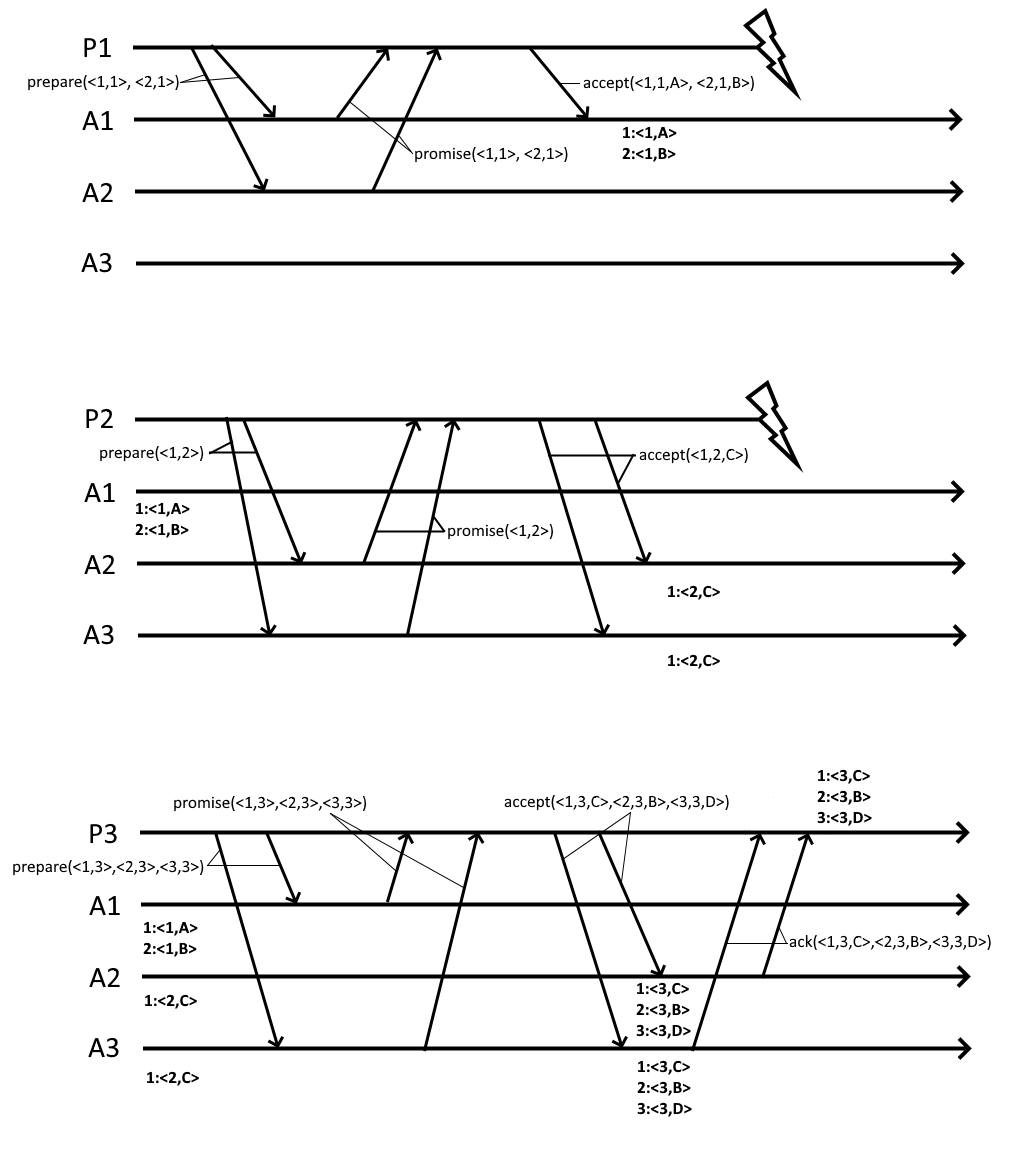
\includegraphics[width=\linewidth]{img/paxos_fail_2.png}
	\caption{Randfall von Paxos, bei dem sich die Reihenfolge von Zustandsänderungen ändern kann, nachdem sie bereits in einer anderen Reihenfolge von einen Proposer vorgeschlagen wurden. P1 schlägt die Werte A und B für die Indizes 1 und 2 vor. P3 schlägt jedoch die Werte C und B für die Indizes 1 und 2 vor und bekommt dafür eine Mehrheit. B könnte jedoch von A abhängig sein, da die Werte in dieser Reihenfolge von P1 vorgeschlagen wurden.}
	\label{fig:paxos_fail}
\end{figure}

\begin{figure}[H]
	\centering
	\includegraphics[width=\linewidth]{img/zab.png}
	\caption{Ablauf von Zab.}
	\label{fig:zab}
\end{figure}


Zab läuft im Gegensatz zu Paxos in drei Phasen ab (siehe \ref{fig:zab}):
\begin{enumerate}
	\item \textbf{Discovery}: Durch einen beliebigen Leader-Election-Algorithmus wird ein Kandidat für den Leader bestimmt. Alle anderen Server sind Follower. Alle Follower senden eine Nachricht mit der höchsten \textit{Epoch}-Nummer, die sie erhalten haben, an den Kandidaten. Wenn der Kandidat die \textit{Epoch}-Nummer von einer Mehrheit der Follower erhalten hat, schlägt er eine \textit{Epoch}-Nummer vor, die höher ist als alle, die er erhalten hat. Die Follower akzeptieren wiederum die vorgeschlagene \textit{Epoch}-Nummer und senden zusätzlich ihre History (das Log mit den bereits vorhandenen Transaktionen).
	Die Phase wird erst beendet, sobald alle Follower die \textit{Epoch}-Nummer akzeptiert haben und der Leader die History aller Follower erhalten hat. Nun kann der Leader die aktuellste History bestimmen und diese in der nächsten Phase auf alle Follower replizieren. Durch die Discovery-Phase wird sichergestellt, dass die Follower keine kleinere \textit{Epoch}-Nummer akzeptieren.
	\item \textbf{Synchronization}: Der Kandidat schlägt sich selbst als Leader vor und sammelt Stimmen dafür ein. Dabei sendet der Leader auch die in der Discovery-Phase gewählte History, die auf die Follower repliziert wird. Wenn der Kandidat ein Quorum hat, wird er zum Leader und sendet eine \textit{Commit}-Nachricht an die Follower, die den Leader als gewählt anerkennen können und die Transaktionen in der vorher gesendeten History ausführen können. Durch diese Phase wird sichergestellt, sich die Server auf die History geeinigt haben und diese nicht mehr durch einen neuen Leader gelöscht werden kann.
	\item \textbf{Broadcast}: Der in der Synchronization-Phase etablierte Leader sendet neue Transaktionen an die Follower und sendet eine \textit{Commit}-Nachricht mit der Transaktion an alle Follower, sobald die Transaktion auf einer Mehrheit der Follower repliziert wurde. Sobald die Follower eine \textit{Commit}-Nachricht erhalten, können sie die entsprechende Transaktion ausführen. Diese Phase läuft ähnlich dem 2-Phase-Commit-Protokoll \cite{pc} ab. Die Verbindungen zwischen Leader und Followern wird über Heartbeats überwacht. Sobald ein Follower die Verbindung zum Leader verliert, startet er die Discovery-Phase. Wenn ein Leader die Verbindung zu einer Mehrheit der Server verliert, startet er ebenfalls die Discovery-Phase und gibt dadurch seine Leadership ab.
\end{enumerate}

\subsection{Raft}

Raft \cite{raft, raft-thesis} basiert ebenso wie Paxos auf dem Replicated-State-Machine-Modell basiert. Die Autoren begründen die Entwicklung von Raft damit, dass Paxos schwierig zu verstehen und zu implementieren sei. Deswegen wollten sie einen einfacheren Algorithmus entwickeln, der auf dem selben Modell basiert. Raft geht ebenso wie Paxos von einem Crash-Recovery-Modell und einem unzuverlässigen Netzwerk aus.
Im Gegensatz zu Paxos wird das Einigungsproblem bei Raft in drei Teilprobleme aufgeteilt:
\begin{itemize}
	\item \textbf{Leader Election}: Die Wahl eines Leaders ist bei Raft fester Bestandteil des Algorithmus 
	\item \textbf{Log Replication}: Das Log mit den Befehlen muss vom Leader auf die anderen Server des Cluster repliziert werden und es muss sich auf eine Reihenfolge geeinigt werden.
	\item \textbf{Safety}: Es muss Folgendes gelten: Alle Befehle müssen von allen Zustandsmaschinen in der gleichen Reihenfolge ausgeführt werden.
\end{itemize}

\subsubsection{Leader Election}

Ein Server hat immer einen der States \textit{Follower}, \textit{Candidate} oder \textit{Leader}. Alle Server starten als Follower. Raft teilt die Zeit in \textit{Terms} auf, die fortlaufend nummeriert werden. Jeder Term beginnt mit der Wahl eines Leaders. Jeder Server speichert seinen aktuellen Term und tauscht ihn bei jeder Kommunikation mit den anderen Servern aus. Wenn ein Server eine Anfrage mit einem alten Term bekommt, dann lehnt er diese ab. Wenn er eine Anfrage mit einem höheren Term bekommt, übernimmt er diesen und wird zum Follower. Eine Leader Election wird gestartet, wenn ein Follower eine Zeit lang keinen Heartbeat von einem Leader bekommt. Er wird dann zu einem Candidate und versucht Leader zu werden. Dabei startet er einen neuen Term, indem er seinen gespeicherten Term inkrementiert. Er sendet dann Vote Requests an alle anderen Server. Diese geben dem, Candidate ihre Stimme, falls sie ihre Stimme nicht bereits im selben Term einem anderen Server gegeben haben. Falls der Candidate von der Mehrheit der Server eine Stimme erhalten hat, wechselt er seinen Status zum Leader. So ist sichergestellt, dass es in einem Term maximal einen Leader geben kann. 

Es kann jedoch passieren, dass es in einem Term keinen Leader gibt. Falls mehrere Follower im gleichen Term eine Wahl starten (falls der Timer, der die letzte Nachricht von einem Leader überwacht, etwa zur gleichen Zeit ausläuft), kann es sein, dass es keine Mehrheit für einen Kandidaten gibt. Dann beginnen ein oder mehrere Candidates einen neuen Term und starten eine neue Wahl. Damit solche Konflikte selten vorkommen, sollten die Timeouts randomisiert werden, sodass es unwahrscheinlich ist, dass mehrere Server gleichzeitig eine Wahl starten.

Sobald ein Server sich zum Leader ernannt hat, kann er Anfragen von Clients bearbeiten und sendet periodisch Heartbeats an alle Follower, um seine Leadership aufrecht zu erhalten.

\subsubsection{Log Replication}

Im normalen Betrieb, d.h. ohne Leaderwechsel, nimmt der Leader Client-Anfragen an, schreibt diese ins Log und versucht sie, auf die Follower zu replizieren. Dazu sendet er sogenannte Append Entries Requests mit den Einträgen, die er replizieren möchte, an die Follower. Die Follower fügen diese in ihr eigenes Log ein und senden eine Bestätigung zurück, falls dies erfolgreich durchgeführt wurde. Der Leader merkt sich für jeden Follower einen \textit{Match Index}, der angibt, bis zu welchem Eintrag das Log des Followers dem des Leaders entspricht. Dadurch kann er feststellen, wann ein Eintrag auf eine Mehrheit der Server repliziert wurde. Sobald dies der Fall ist, kann er den Eintrag seiner State Machine übergeben und ausführen. Dann kann eine Antwort an den Client gesendet werden. Mit dem nächsten Append Entries Request oder Heartbeat wird der \textit{Commit Index} an die Follower weitergegeben, sodass diese den Eintrag ebenfalls ausführen können.

Nach einem Leader-Wechsel muss der Leader die Logs der Follower seinem eigenen Log angleichen. Dafür speichert er sich für jeden Follower einen \textit{Next Index}, der angibt, welcher Eintrag als nächstes an diesen Follower gesendet werden soll. Nach der Wahl zum Leader wird dieser für alle Follower auf den Index des letzten Eintrags initialisiert. Der Leader sendet außerdem bei jedem Append Entries Request den Term des letzten Eintrags, der vor den gesendeten Einträgen im Log ist, mit. Follower lehnen ein Append Entries Request ab, falls dieser Term nicht mit dem Term des Eintrags an diesem Index in ihrem Log übereinstimmt. Dann muss der Leader den \textit{Next Index} dieses Followers dekrementieren und es nochmal versuchen. Falls diese Überprüfung beim Follower nicht fehlschlägt und bereits inkonsistente Einträge vorhanden sind, werden alle folgenden Einträge gelöscht, sodass das Log dann bis zum Index des letzten gesendeten Eintrags dem des Leader entspricht.

\subsubsection{Safety}

Die zentrale Eigenschaft, die gelten muss damit das System korrekt funktioniert, ist: Sobald ein Log-Eintrag von einer State Machine ausgeführt wurde, darf keine andere State Machine auf einem anderen Server einen anderen Befehl für diesen Log-Eintrag ausführen. Dadurch wird offensichtlich sichergestellt, dass alle State Machines die Befehle in der gleichen Reihenfolge bearbeiten. Diese Eigenschaft ist in Raft äquivalent zu: Wenn ein Leader entscheidet, dass ein Eintrag \textit{committed} ist und diesen der State Machine übergibt, dann muss dieser Eintrag in den Logs aller zukünftigen Leadern vorhanden sein. Dies wird durch zusätzliche Einschränkungen beim Committen und bei der Leader Election erreicht.

\begin{itemize}
	\item \textbf{Leader Election}: Die Candidates senden mit ihren Vote-Requests den Term und Index des letzten Eintrags ihres Logs mit, anhand derer die wählenden Server entscheiden, ob sie dem Candidate ihre Stimme geben oder nicht. Damit Log Einträge, die auf einer Mehrheit der Server repliziert sind, nicht gelöscht werden, gibt der Server dem Candidate keine Stimme, falls sein Log kompletter ist, d.h. falls der Term des letzten Eintrags größer ist oder falls der Term gleich ist und der Index größer ist. Dadurch hat der nächste Leader dann das kompletteste Log unter einer Mehrheit der Server.
	\item \textbf{Commit}: Um einen Eintrag zu committen, muss mindestens ein Eintrag aus dem aktuellen Term des Leaders auf einer Mehrheit der Server repliziert worden sein. Sonst kann es passieren, dass ein Server Leader wird, der die auf einer Mehrheit replizierten Einträge nicht in seinem Log hat, da er nur neuere Einträge in seinem Log hat. Abbildung \ref{fig:zab} zeigt einen solchen Fall: Die Einträge in Index 2 und 3 mit Term 2 sind auf einer Mehrheit der Server repliziert. Falls Server 2 jedoch Leader in Term 4 wird, darf er diese Einträge nicht committen. In Term 5 kann Server 1 Leader werden, da er das längste Log hat. Er würde dann die Logs der Follower seinem anpassen und die Einträge mit Term 2 würden gelöscht werden. Sobald Server 2 jedoch einen Eintrag in seinem aktuellen Term (Term 4), auf Server 3 repliziert hat, kann Server 1 nicht mehr in Term 5 Leader werden. Jetzt können die Einträge in den Indizes 2-4 committet werden.
\end{itemize}

\begin{figure}[H]
	\centering
	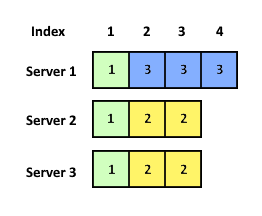
\includegraphics{img/raft-log.png}
	\caption{Log-Einträge von drei Raft-Servern. Die Zahl in den Einträgen gibt den Term des Eintrags an.}
	\label{fig:zab}
\end{figure}